

\section{Somaïr}
Dans cette partie, nous allons tout particulièrement nous intéresser au fonctionnement de Somaïr, la mine à ciel ouvert d'Orano au Niger, car c'est la qu'est déployé le projet CanOp et qui me faut comprendre leur procédure pour donner des suggestions cohérentes.
\subsection{L'exploration}
Avant le début de l'extraction, des géologues ont réalisé des études pour trouver d'éventuel gisement. S'ils soupçonnent la présence d'uranium, les géologues vont réaliser des campagnes de sondage successives\footnote{Soit une carotte ou un forage dans lequel on abaisser un 
sonde gamma. Cela permet d'etablire le gisment en 3D}. La maille de sondage sera à affiner jusqu'à avoir des forages espacés de 25~m. 
\subsection{L'extraction}
\label{ssec_extraction}
Si la décision de passer en production est prise alors on va venir enlever toute la roche au-dessus du gisement (50 a 70~m à Somaïr) et l’on va affiner le sondage jusqu'à une maille de 5~m*5~m qui va permettre de modéliser au mieux la distribution d'uranium dans le sol. Enfin, la fosse sera divisée en carrés de 2,5~m de large sur 2,5~m de longueur sur 0,5~m de profondeur que l'on appellera "slab" par la suite. Pour extraire ces slabs, on enterre juste assez d'explosif pour fragiliser la roche et permettre qu'une pelle mécanique puisse extraire la slab pour la charge dans un camion.
\subsection{Classification des slabs}
\label{ssec_classification}
\begin{figure}
    
    \begin{subfigure}[t]{0.4\textwidth}
        \centering
        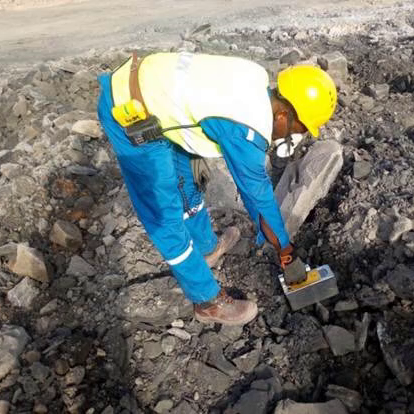
\includegraphics[height=0.3\paperwidth]{img/photo/Travail_geiger.png}
        \caption{Photo d'un operateur utilisant un compteur Geiger Müller pour mesurer la teneur en uranium d'un slab}
        \label{fig_AP_geiger}
    \end{subfigure}
    \begin{subfigure}[t]{0.6\textwidth}
        \centering
        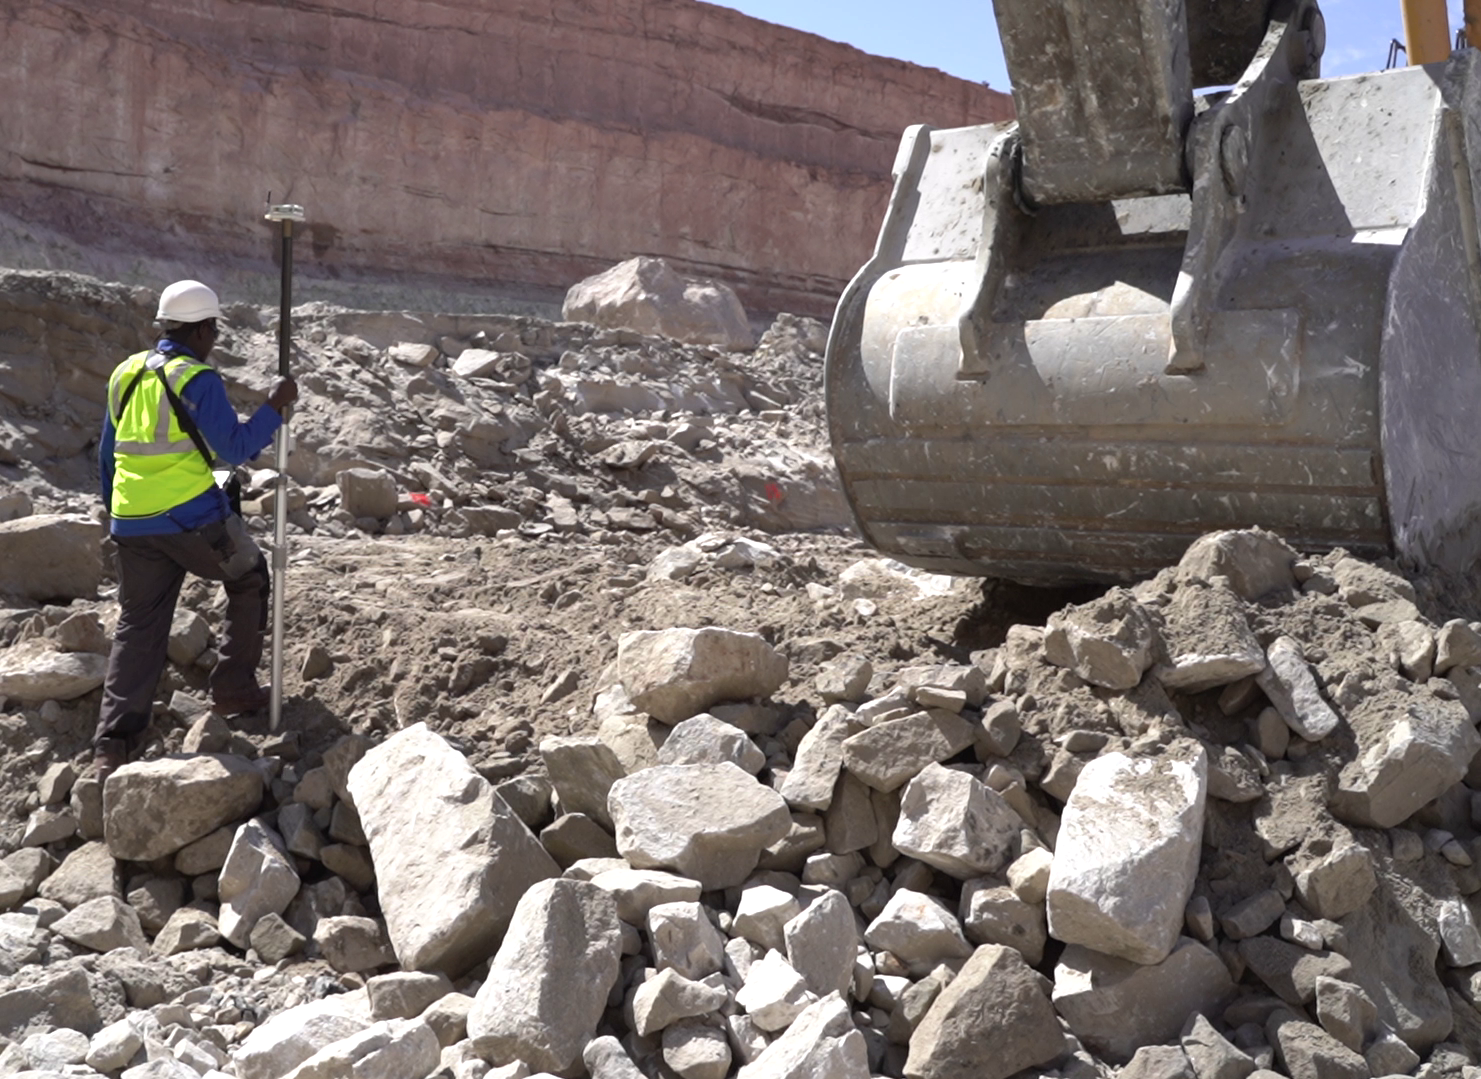
\includegraphics[height=0.3\paperwidth]{img/photo/CanOp_utilisation.png}
        \caption{Photo d'un operateur utilisant la CanOp pour mesurer la teneur en uranium d'un slab. Il porte une tablette pour voir les mesure et sa position en temps reel}
        \label{fig_AP_CanOp}
    \end{subfigure}
    \caption{Photo d'AP utilisant un compteur Geiger Müller et la CanOp}
\end{figure}
Pour savoir comment traiter ces slabs  après extraction, nous les catégorisons en 7~classes de M0 à  en fonction de leur teneur en uranium. Au début, ces teneurs étaient mesurées  Les slabs~M0 sont dites stériles, car elle contient tellement peu d'uranium que l'on ne souhaite pas les traiter. Les classes~M1 et M2 subissent un traitement que l'on dit statique, car c'est slab sont empiler et l’on attend que l'uranium descend par gravité jusqu'un bas. Enfin les slabs de classe supérieure reçoivent un traitement dynamique où en fonction de leur classe elles seront dissoutes avec plus ou moins d'acide selon leurs classes. Il est donc important de bien classer les slabs, car sinon, soit on gaspille  de l'acide ou alors il reste des l'uranium non extrait dans notre refus.
%TODO:mistakes
Avant, pour classer une slab, un Aide Prospecteur (AP) utiliser un compteur Geiger Müller en se penchant pour obtenir des mesures a plusieurs points sur le slab. Il était donc pénible de se pencher en permanence et donc en 2018 a été lancer le projet CanOp pour réduire la pénibilité de la tache.
